\documentclass{olplainarticle}
\usepackage{hyphenat}
% Use option lineno for line numbers 
\setlength{\parindent}{0pt}
\setlength{\parskip}{6pt}
\usepackage{xcolor}
\colorlet{color2}{white}  % olplainarticle uses color2 for abstract text
\usepackage{tikz}
\usetikzlibrary{positioning}
\definecolor{GTNavy}{HTML}{003057}
\definecolor{GTGold}{HTML}{B3A369}
\definecolor{GTLight}{HTML}{F5F1E6}
\bibliographystyle{unsrtnat}
\usepackage[colorlinks=true,linkcolor=blue,citecolor=blue,urlcolor=blue]{hyperref}
\usepackage{subcaption}
\usepackage{graphicx}
\usepackage{float}
\usepackage{listings}
% \usepackage{xcolor} % Removed duplicate import
\usepackage{tikz}
\usetikzlibrary{shapes.geometric, arrows, positioning}

% \title{CSE 6010 Final Project Report: BuzzNav System}

% \author{Chia-Hsin Chiu, Ming-Cheng Fan, Jing He, Haowen Jiang, Fred Yang\thanks{Authors are listed in alphabetical order.}}


\usepackage[numbers,sort&compress]{natbib}
\makeatletter
\makeatother
\begin{document}
% ===================================================================
%                           COVER PAGE
% ===================================================================
\begin{titlepage}
    \centering
    \vspace*{1cm}

    % 1. Project Title 
    {\Huge \textbf{CSE 6010 Final Project Report: \\
    BuzzNav System}}

    \vspace{1.5cm}

    {\Large \textbf{Group Number: 6}}

    \vspace{2cm}

    % 4. Team Members 
    {\Large \textbf{Team Members:}} \\
    \vspace{0.5cm}
    {\large
    Chia-Hsin Chiu\\
    Ming-Cheng Fan\\
    Jing He\\
    Haowen Jiang\\
    Fred Yang
    }

    \vspace{2.5cm}

    % 5. GitHub Repository Link 
    {\Large \textbf{GitHub Repository:}} \\
    \vspace{0.5cm}
    \url{https://github.com/fredkyang/cse6010-buzznav}
    \vfill
    % 6. Recording Link 
    {\Large \textbf{Recording Link:}} \\
    \vspace{0.5cm}
    \url{https://drive.google.com/file/d/1x6ugIPxoyecRRnZMM4Qze4Fk-Sp_C6E-/view?usp=share_link}

    \vfill
    
    % Course Info & Date [cite: 3]
    {\large
    CSE 6010: Computational Problem Solving \\
    Georgia Institute of Technology \\
    December 8, 2025
    }

\end{titlepage}

% ===================================================================
%                       MAIN REPORT CONTENT
% ===================================================================
\newpage
\setcounter{page}{1}

\flushbottom
% \maketitle

% GitHub: \href{https://github.com/fredkyang/cse6010-buzznav}{GitHub repository}


\section*{abstract}
The Georgia Tech (GT) campus holds meaningful memories for many people, but it is not easy for students and visitors to quickly locate buildings and navigate through multiple destinations. Therefore, we built BuzzNav, a GT campus navigation system.
Three routing algorithms are implemented in the system: the A algorithm* for point-to-point navigation, a parallelized A algorithm* for sequential via-point routing, and TSP optimization (for unordered multi-destination planning) using dynamic Held-Karp planning. Our team utilized parallel computation (OpenMP) and separately achieved a 7.2x speedup on Dijkstra distance matrix calculation and a 3.8x speedup on via-point path planning.
The website (built on Leaflet.js and Flask) includes accessible and convenient functions: interactive map visualization, auto-complete search, dynamic multi-point management, and turn-by-turn navigation instructions.
Our implementation has proven that BuzzNav is a speedy and practical navigation system.

\section*{Notations}
Unless otherwise stated, we use the following notations throughout this work:

\begin{itemize}
    \item $n$: the total number of nodes in the graph.
    \item $V$: the total number of edges in the graph.
    \item $k$: the number of target nodes that must be visited.
    \item $v_i$: the $i$-th node in the graph.
\end{itemize}

\section{Data Acquisition and Preprocessing}
Our data are obtained from \textbf{OpenStreetMap (OSM)}, an open geospatial platform collaboratively maintained and continuously updated by contributors worldwide. OSM organizes geographic information in a structured format consisting of \textbf{nodes}, \textbf{ways}, and \textbf{relations}:
\begin{itemize}
    \item \textbf{Buildings} are represented as closed polygons, defined by a series of latitude–longitude coordinates (nodes). Each building polygon is associated with descriptive tags, such as \texttt{building=yes} and \texttt{name=Tech Tower}.

    \item \textbf{Roads} are represented as polylines (collections of line segments) defined by ordered nodes. Road attributes include type (e.g., \texttt{highway=primary}, \texttt{highway=residential}) and access restrictions (e.g., \texttt{network\_type=drive}).
\end{itemize}


For simplicity, we extracted \textbf{motor-vehicle-accessible roads} (\texttt{network\_type=drive}) within the Georgia Tech campus.

\subsection*{Processing Steps}
\begin{enumerate}
    \item \textbf{Road and Building Data Processing}
\begin{itemize}
    \item Download road and building data from OSM, keeping only motor-vehicle-accessible roads and the target buildings.
    \item Simplify road geometries and compute the geometric centroid of each selected building.
\end{itemize}
    
    \item \textbf{Projection onto Roads}
    \begin{itemize}
        \item For each building centroid, compute the shortest distance to every road segment using point-to-segment projection.
        \item Identify the nearest road segment and project the centroid orthogonally onto it, yielding a projection point.
    \end{itemize}
    
    \item \textbf{Graph Update}
    \begin{itemize}
        \item Insert the projection point as a new node in the road graph.
        \item Split the corresponding road edge into two segments: from the original road start node to the projection point, and from the projection point to the road end node. Update the edge lengths using great-circle (haversine) distances.
        \item Record the mapping between each building and its associated projection node.
    \end{itemize}
    
    \item \textbf{Adjacency List Construction}
    \begin{itemize}
        \item For each node $i$, explicitly store its \textbf{neighbors}, i.e., the set of adjacent nodes directly connected to $i$.
        \item Each neighbor entry is stored together with the corresponding edge distance $d_{ij}$.
    \end{itemize}
\end{enumerate}


\section{Project description}
The system allows users to input an arbitrary number of building names. After converting these names into node id, the program selects an appropriate routing algorithm based on the number of locations. 

The flow chart is shown as Figure~\ref{fig:flowchart}. When exactly two locations are provided, the system executes the A* algorithm to compute the shortest path between the source and destination. When more than two locations are given, the via-point routing algorithm is triggered, which performs parallel A* searches between consecutive viapoints. If more than two locations are provided and the optimization mode is enabled, the system instead formulates and solves a Traveling Salesman Problem (TSP). This algorithm first parallelizes Dijkstra's algorithm to obtain all-pairs shortest paths, then applies the Held--Karp dynamic programming algorithm to compute the optimal visiting order. The output for all modes includes the visiting sequence of the requested nodes, the total travel distance, a plotted route on the web-based campus map, and automatically generated turn-by-turn directions.

\begin{figure}[h]
  \centering
  \includegraphics[width=0.9\linewidth]{docs/Final Project Report/flowchart.png}%
  \caption{Program logic of the BuzzNav routing engine. 
  Given user-specified building names, the system either computes a shortest path
  between two locations using A* or, when route optimization is enabled, applies
  a TSP-based solver and via-point A* module to generate the visit order, total
  distance, map visualization, and turn-by-turn directions.}
  \label{fig:flowchart}
\end{figure}


\paragraph{Continuous Integration.}
In the GitHub team collaborative project, automated builds with Actions are necessary to guarantee code quality and project safety. The CI pipeline compiles the project with GCC-13 on every push, giving timely feedback to every editor and preventing failed code into the main codebase.


\section{Literature Review}
Navigation systems improve mobility by helping users reach destinations efficiently while reducing uncertainty. For constrained environments like university campuses, OpenStreetMap (OSM) provides open-source road and building data suitable for routing applications \cite{10.1007/978-3-642-10601-9_13, s18020509}. Campus navigation prototypes show its adaptability for small-scale routing.

Most navigation systems use graph-based models, representing intersections and roads as nodes and edges. Buildings are linked via geometric techniques, such as centroid projection, to the network \cite{Map-mappingResearch}. Shortest-path algorithms like Dijkstra and A* compute efficient routes, with A* leveraging heuristics for faster performance \cite{madkour2017survey}.

Generating intuitive navigation instructions is crucial. Effective guidance identifies decision points, turning angles, and translates them into simple directions, sometimes using landmarks to reduce disorientation \cite{RICHTER2008233}. Overall, campus-scale navigation using OSM, graphs, and classical algorithms is feasible, with future improvements possible through landmarks or augmented reality.

\section{Coding Strategy}

\subsection{A* Algorithm}

To address the requirement for a point-to-point shortest path calculation, we used A* search algorithm rather than Dijkstra because that while Dijkstra guarantees the shortest path, it searches uniformly in all directions, causing unnecessary computations and time waste. 

In contrast, A* includes a heuristic function ($h(n)$)—Euclidean distance in our implementation—served as the estimated cost to the goal node, which could effectively guide the search direction and thus reduce the search space. We implemented the solution using a min-priority queue binary heap to retrieve the node with the lowest $f(n)$ score. 

The primary trade-off of this approach is increased memory complexity (space) required to maintain the open and closed sets compared to simpler greedy algorithms or iterative deepening. However, we accepted this spatial cost to secure the guarantee of optimality and completeness that a pure Greedy Best-First Search cannot provide, achieving the necessary balance between execution speed and path accuracy.

\subsection{Via Points }

\paragraph{Problem Motivation.}
In the real-world navigation scenarios, users often visit one or several intermediate points before they arrive at their final goal point. Let's use two familiar cases from college experience. Professor may not go straight to classroom for class. Instead, they will buy a cup of coffee after leaving office and then walk to the classroom. After class,students may visit several places, like cafeteria, school post office, library and lab, and then go back to dorm to rest. For better meet these similar needs, we create the second function: via point which  enables users to free choose one or more intermediate points.

\paragraph{Design Decision: Segment Decomposition.}
The scenarios mentioned above can be simplified into the following model: Finding out the shortest path from a start location $s$ to a destination $d$ while going through some intermediate points  $v_1, v_2, \ldots, v_k$ in order. So let's seek:
\[
    s \to v_1 \to v_2 \to \cdots \to v_k \to d
\]

We break this into $(k+1)$ separate routing sub-problems:
\begin{itemize}
    \item Segment 1: $s \to v_1$
    \item Segment 2: $n_1 \to v_2$
    \item $\vdots$
    \item Segment $k+1$: $v_k \to d$
\end{itemize}

Each segment is solved independently and parallelly through reusing A*.

\paragraph{Rationale.}
This decomposition strategy brings several advantages to BuzzNav;
\begin{itemize}
    \item \textbf{Parallelizability}: Each segment like $v_i \to v_{i+1}$ is independent from other. So that all segment can be solved simultaneously.
    \item \textbf{Scalability}: As the number of via points grows, the complexity increase linearly.
    \item \textbf{Reusability}:Each segment is a standard two-point path planning, which can directly reuse A* without modification.
    \item \textbf{Optimality}: Because every segment finds the shortest path, the final total optimal path can be found by joining these segments sequentially.
\end{itemize}

\paragraph{Tradeoffs.}
 The primary limitation is requiring the predetermined visit order. If a user only care about visiting a set of via points without order constraints, this method maybe lead to suboptimal results compared to TSP optimization. However, when is comes to the scenarios where the sequence matters (like scheduled visiting plan), this decomposition is both efficient and appropriate.

\paragraph{Parallelization}
For accelerating computation, we adopt OpenMP to execute independent segment search tasks in parallel. By distributing $(n+1)$ A* function calls across CPU cores, computational time cost is hugely decreased when dealing with many via points.

\subsection{TSP}
First, unordered traversal of a given set of nodes corresponds to a classical Traveling Salesman Problem (TSP).A straightforward brute-force approach is to enumerate all possible visiting
orders of the $k$ selected target nodes. Since there are $k!$ permutations
and each evaluation requires checking the $k$ transitions along that order,
the traversal alone incurs a cost of $O(k \cdot k!)$.

However, this does not include the cost of constructing the pairwise shortest‐path
table between these $k$ nodes. Suppose the full campus graph contains
$V$ nodes and $E$ edges. Computing all $k \times k$ shortest distances requires
running Dijkstra’s algorithm $k$ times, which costs $O(k \cdot E \log n)$.

Given that this brute-force method is computationally prohibitive, we
instead adopt the classical Held–Karp dynamic programming algorithm
to obtain the optimal route much more efficiently.

We represent each state using a bitmask $S \subseteq \{0,1,\dots,k-1\}$
indicating the set of visited nodes, and an endpoint $i \in S$ denoting
that the tour ends at node $i$. The DP table stores the minimum cost of
visiting all nodes in $S$ and finishing at $i$:
\[
    \mathrm{dp}[S][i].
\]

The DP recurrence is:
\[
    \mathrm{dp}[S][i]
    = 
    \min_{j \in S,\, j \neq i}
    \left(
        \mathrm{dp}[\, S \setminus \{i\}\,][j] + d_{j,i}
    \right),
\]
where $d_{j,i}$ is the shortest-path distance between targets $j$ and $i$.

Using the dynamic programming update formula above, the state space is gradually expanded. 
The initial condition is given by
\[
\mathrm{dp}[\{i\}][0] = 0.
\]
As the size of \(S\) increases, after a finite number of expansions the set \(S\) eventually contains all nodes that must be visited. 
At that point, 
\[
\max_i \; \mathrm{dp}[\{1,2,\ldots,n\}][i]
\]
corresponds to the length of the optimal route, and the associated sequence of visited nodes gives the optimal visiting order. 
Once this order is obtained, the final optimal path can be constructed simply by concatenating the pairwise shortest paths between each pair of consecutive nodes.

\paragraph{How do we derive this recurrence?}
The recurrence relation follows directly from the definition of
$\mathrm{dp}[S][i]$, which denotes the minimum cost of starting from
the designated root node, visiting all nodes in the subset $S$, and
ending at node $i$.

To compute this value, we consider the last step of any such path.
Let $j$ be the node visited immediately before $i$. Since $i$ is the
final node, it must hold that $j \in S$ and $j \neq i$.
If the last segment of the tour is $j \rightarrow i$, then by the time
the path reaches $j$, it must have already visited every node in
$S \setminus \{i\}$ and ended at $j$.

Thus, the cost of completing the entire tour by appending the final edge
$j \rightarrow i$ is:
\[
    \mathrm{dp}[\, S \setminus \{i\} \,][j] + d_{j,i},
\]
where $d_{j,i}$ denotes the distance from $j$ to $i$.

Since the choice of $j$ is not unique, we take the minimum over all
possible predecessors $j$ to obtain the Held--Karp recurrence:
\[
    \mathrm{dp}[S][i]
    =
    \min_{j \in S,\; j \neq i}
    \left(
        \mathrm{dp}[\, S \setminus \{i\} \,][j] + d_{j,i}
    \right).
\]

This derivation highlights the optimal substructure of the TSP:
every optimal tour ending at $i$ can be decomposed into an optimal
subtour ending at some $j$, followed by the final transition from $j$ to $i$.



\paragraph{Parallelization}
To further improve performance, we parallelize the computation of the
pairwise distance table. Specifically, for $k$ selected target nodes, we
must run Dijkstra $k$ times, each from a different source. These
invocations are completely independent and therefore ideally suited for
parallel execution. By assigning each Dijkstra run to a separate thread
using OpenMP, we significantly reduce the wall-clock time required to
construct the full $k \times k$ distance matrix.

\section{Simulator}

Our core algorithms include A*, via-point routing, and TSP computation. Also, we implement the webpage map visualization served as the frontend of BuzzNav. 

\subsection*{A* Algorithm}
The A* algorithm forms the core of the single-pair shortest-path computation and is reused parallelly in the via-point routing. In terms of A* algorithm's concept, it combines the exact cost accumulated so far, denoted as $g(n)$, with the heuristic estimate $h(n)$ of the remaining distance to the goal. In our implementation, the main function \texttt{astar()} maintains a priority queue of frontier nodes, ordered by the evaluation function
\[
    f(n) = g(n) + h(n),
\]
and expands nodes in increasing order of $f(n)$ until the destination is reached. Neighbor distances are updated through standard relaxation rules, and parent pointers are recorded to facilitate reconstruction of the optimal path once the search terminates.

\subsubsection{Complexity Analysis}
\paragraph{Time Complexity}
The time complexity of A* is heavily dependent on the quality of the heuristic function. In the worst-case scenario, where the heuristic is monotonic but provides minimal guidance (approximating Dijkstra's algorithm), the algorithm may visit all nodes and edges. With the graph represented as an adjacency list and the priority queue implemented as a binary heap, the worst-case time complexity is $O(E \log V)$, where $V$ is the number of vertices and $E$ is the number of edges. The logarithmic factor arises from the \texttt{extract-min} and \texttt{decrease-key} operations within the priority queue.

\paragraph{Space Complexity}
The space complexity is determined by the need to store the search frontier (open set) and the path reconstruction history (closed set/parent pointers). Unlike Iterative Deepening Search, A* must keep all generated nodes in memory to prevent cycles and avoid redundant computations. In the worst case, where the algorithm explores the entire graph before finding the target (or if the target is unreachable), the space complexity is $O(V)$, as every vertex is eventually stored in the auxiliary data structures.
\subsection{Via-Point Routing Algorithm}

Based on the A*, via point algorithm handles multi via point navigation by computing and merging independent path segments.

\paragraph{Structure.}
Given a start point $s$, destination node $d$, and ordered via points  $n_1, n_2, \ldots, n_k$, the algorithm will proceed in 3 steps:

\textit{Step 1: Segment Identification.}
We build $(k+1)$ routing planning segment corresponding to consecutive nodes:
\[
\text{Segments} = \{(s, n_1), (n_1, n_2), \ldots, (n_{k-1}, n_k), (n_k, d)\}
\]

\textit{Step 2: Parallel Optimization.}
For every segment $(u,v)$, we apply A* to find the shortest path. This part is parallelized by OpneMP's parallel-for directive. Each segment will be solved on different Cores. By the way, the number of segments equal the degree of parallelism.

\textit{Step 3: Merge path.}
After computing all segments, nodes will be connected one after another by order, forming a complete path. Besides, in this way, redundant nodes will be omitted or skipped.

For example, if $j$ segment's completed path $[e,r,t]$ and $k$ segment's completed path $[t,y,u]$, the merged result is $[e,r,t,y,u]$ instead of $[e,r,t,t,y,u]$.

\paragraph{Why do this.}
Reusing A* is because of the following reasons:
\begin{itemize}
    \item A* is already succeeded and validated 
    in direct path scenarios.
    \item Each segment is an independent and standard 2 points shorest path planning.
\end{itemize}
 There is another alternative modified A* while keeping node order constraint. However, this has to add an additional state management function to trace via points(visited or not) and is unable to parallel easily. Overall, the decomposition strategy is superior to the modified A*, as it is more efficient and straightforward.

\paragraph{Complexity Analysis.}

\textbf{Time Complexity.}  
There are $n$ via points , $v$ nodes and $E$ edges in a graph. So the complexity is:
\[
    O((n+1) \cdot E \log V)
\]
As each segment A* search requires $O(E \log V)$ time to use a binary heap priority queue.

Luckily, with parallelization on $(n+1)$ cores, computational time cost deceased dramatically:
\[
    O(E \log V)
\]
This is theoretical improvement effect, while the practical performance depends on system resources and load balance.


\textbf{Space Complexity.} 
Each segment can store up to $V$ nodes theoretically. Hence, the total space before merging is:
\[
    O((n+1) \cdot V)
\]
After merging, the complete path will less than $(n+1) \cdot V$ (Practically, it will be much shorter. )

\paragraph{Thread Safety.}
Unlike simple sequential computing, parallel computing requires extra steps to ensure correctness.
\begin{itemize}
    \item Every thread operates on corresponding segment, which has it own independent memory allocations.
    \item The graph structure shared across all threads but in read-only mode is able to eliminate race conditions.
    \item To avoid write conflicts, the result is written to a preassigned location in the array specified by the corresponding segment id.
\end{itemize}

Our lock-free structure not only supports accuracy, but also minimizes synchronization overhead.

\subsection{TSP Algorithm}
In the preprocessing stage, we run Dijkstra's algorithm once for each node that needs to be visited, thereby obtaining the pairwise shortest paths and their corresponding distances.
After this preprocessing step, we no longer need to consider the entire graph; only the $k$ selected nodes and their visiting order matter.

In the TSP solving stage, we use the Held--Karp dynamic programming algorithm. The detailed ideas and implementation have already been explained in the Coding Strategy section, so they are not repeated here.

Finally, once the optimal visiting order is obtained, we stitch together the previously stored shortest-path sequences to form the complete optimal route.

\paragraph{How do we ensure that the route we find is truly optimal?} This is jointly guaranteed by the optimality of Dijkstra's algorithm and the optimality of the Held--Karp algorithm. The correctness of Dijkstra's algorithm has already been covered in class, and the optimality of Held--Karp has been explained in the Coding Strategy section. Our dynamic programming formulation enumerates all possible visiting orders of the selected nodes, so the result it produces must be globally optimal.

\paragraph{Why Dijkstra?}
Our campus graph is sparse, weighted, and contains no negative edges,
making Dijkstra’s algorithm a natural fit. In contrast, the classical
Floyd--Warshall algorithm computes all-pairs shortest paths in
$O(V^3)$ time, which is prohibitively expensive for large graphs where
$V$ (the total number of nodes) may reach the thousands. Although
Floyd--Warshall produces a complete distance matrix in one execution,
its cubic complexity makes it unsuitable for our data scale.

Compared with A*, Dijkstra’s algorithm offers another key advantage in
our setting: a \emph{single} execution computes the shortest-path
distances from the source to \emph{all} other nodes. A* is designed for
single-source \emph{single-target} search and relies on a heuristic
function to guide the exploration. Because our task requires the full
set of distances from each selected building to all others, using A*
would require running it separately for every source--target pair,
resulting in $O(k^2)$ A* calls for $k$ selected buildings. This provides
no benefit over Dijkstra and introduces additional overhead from
heuristic evaluation. Therefore, Dijkstra’s single-source
all-destination property makes it the most appropriate and efficient
choice for constructing the pairwise distance matrix.
\subsubsection{Complexity Analysis}

\paragraph{Time Complexity.}
The overall running time of our approach consists of two major components:
(1) computing the pairwise shortest-path distances among the $k$ selected
nodes, and (2) solving the TSP using the Held--Karp dynamic programming
algorithm.

\textbf{(1) Pairwise shortest-path computation.}
For each of the $k$ selected buildings, we run Dijkstra’s algorithm once.
Given a campus graph with $n$ nodes and $E$ edges, a single Dijkstra run
takes $O(E \log n)$ time using a binary heap. Thus, constructing the
$k \times k$ distance matrix costs:
\[
    O(k \cdot E \log n).
\]

\textbf{(2) Held--Karp dynamic programming.}
The dynamic programming table includes all subsets
$S \subseteq \{0,\dots,k-1\}$ and all endpoints $i \in S$.
For each state $(S, i)$, we search over all possible predecessors $j \in S$,
adding a factor of $k$. Therefore, the time complexity of Held--Karp is:
\[
    O(k^2 2^k).
\]

\textbf{Total time complexity.}
Combining both components, the total running time of the entire algorithm is:
\[
    O\!\left(k \cdot E \log n \;+\; k^2 2^k\right),
\]
where the first term corresponds to shortest-path preprocessing and the
second term corresponds to solving the TSP. For typical campus navigation
applications where $k \le 15$, the DP portion is tractable, while
Dijkstra preprocessing often dominates the runtime.

\paragraph{Space Complexity.}
The total memory usage consists of three components:
the pairwise distance matrix, the stored shortest-path sequences, and
the DP and parent tables used by Held--Karp.

\textbf{(1) Pairwise distance matrix.}
For $k$ selected nodes, the all-pairs shortest-path distances are stored
in a $k \times k$ matrix, which requires:
\[
    O(k^2)
\]
space.

\textbf{(2) Reconstructed shortest-path sequences.}
In addition to the distance values, we store the actual node sequences
for each ordered pair of nodes. The space required(worst case) is:
\[
    O(k^2 n),
\]
.

\textbf{(3) Held--Karp DP and parent tables.}
The dynamic programming table stores one value for each subset
$S \subseteq \{0,\dots,k-1\}$ and each endpoint $i \in S$, requiring:
\[
    O(k 2^k)
\]
memory.  
The parent table, used for reconstructing the optimal tour, stores one
pointer for each DP state and thus requires the same asymptotic space:
\[
    O(k 2^k).
\]

\textbf{Total space complexity.}
Combining all components, the total space usage(worst case) is:
\[
    O\!\left(k^2 n + k 2^k\right).
\]
For typical values of $k$ (e.g., $k \le 15$), the $k 2^k$ term dominates,
while the $k^2$ distance matrix and reconstructed paths remain modest.

\subsection{Webpage Implementation}
\label{sec:frontend}

We built a webpage frontend for users to interact with the pathfinding engine. There are three core values: (1) Location Selection (Start, End, and Via Points), (2) Map Visualization, and (3) Turn-by-Turn Directions.

\subsection{Technology Stack}
We developed the webpage using HTML, CSS, and JavaScript. It connects to the backend via APIs, sending user requests (location selection) and fetching the result (map visualization and turn-by-turn directions).

\subsection{System Integration}
When users launch the navigation, an HTTP request is sent to the API. The request specifies the coordinates (or node IDs) for the start point, end point, and any via points.

\begin{verbatim}
// Example
{
  "start": "College of Computing Building",
  "end": "Student Center",
  "viapoints": ["Howey Building", "Tech Tower"]
}
\end{verbatim}

\section{Results}
\subsection{User Interface and Map Visualization}
When users launch a request, the webpage shows the optimal route for visualization (Fig.~\ref{fig:frontend_overview}).

\subsubsection{Shortest Path Visualization}
Once the input data are received, the shortest path will show on the map. Specifically, the map uses color-coded markers: green for the start point, red for the end point, and yellow for any via points.

\subsubsection{Navigation Instructions}
The webpage also has turn-by-turn directions on the left side. It provides step-by-step guidance for users to know each specific turn and distance.

\begin{figure*}[t]
    \centering
    % Left image
    \begin{minipage}{0.48\textwidth}
        \centering
        \includegraphics[width=\linewidth]{docs/Final Project Report/image1.png}
        
        \caption*{(a) Route Selection}
    \end{minipage}
    \hfill
    % Right image
    \begin{minipage}{0.48\textwidth}
        \centering
        \includegraphics[width=\linewidth]{docs/Final Project Report/image2.png}
        
        \caption*{(b) Navigation Result Visualization}
    \end{minipage}
    \caption{The user interface of BuzzNav. }
    \label{fig:frontend_overview}
\end{figure*}

\subsection{Test Results}
We mainly discuss the performance of the TSP in this section.We tested the TSP functionality and compared it with the ordinary sequential via-point routing. The results show that the optimal route produced by TSP is consistently shorter than that generated by the fixed-order via-point routing. In Fig.~\ref{fig:tsp_comparison}, we consider the route visiting the following locations: \textit{Burger Bowl Field}, \textit{College of Computing Building}, \textit{Scheller College of Business}, \textit{Subway}, \textit{John Lewis Student Center}, and \textit{Tenth and Home Building C}.

% ---------------------- FIGURE PLACEHOLDER ----------------------
\begin{figure*}[t]
    \centering
    % Left image
    \begin{minipage}{0.48\textwidth}
        \centering
        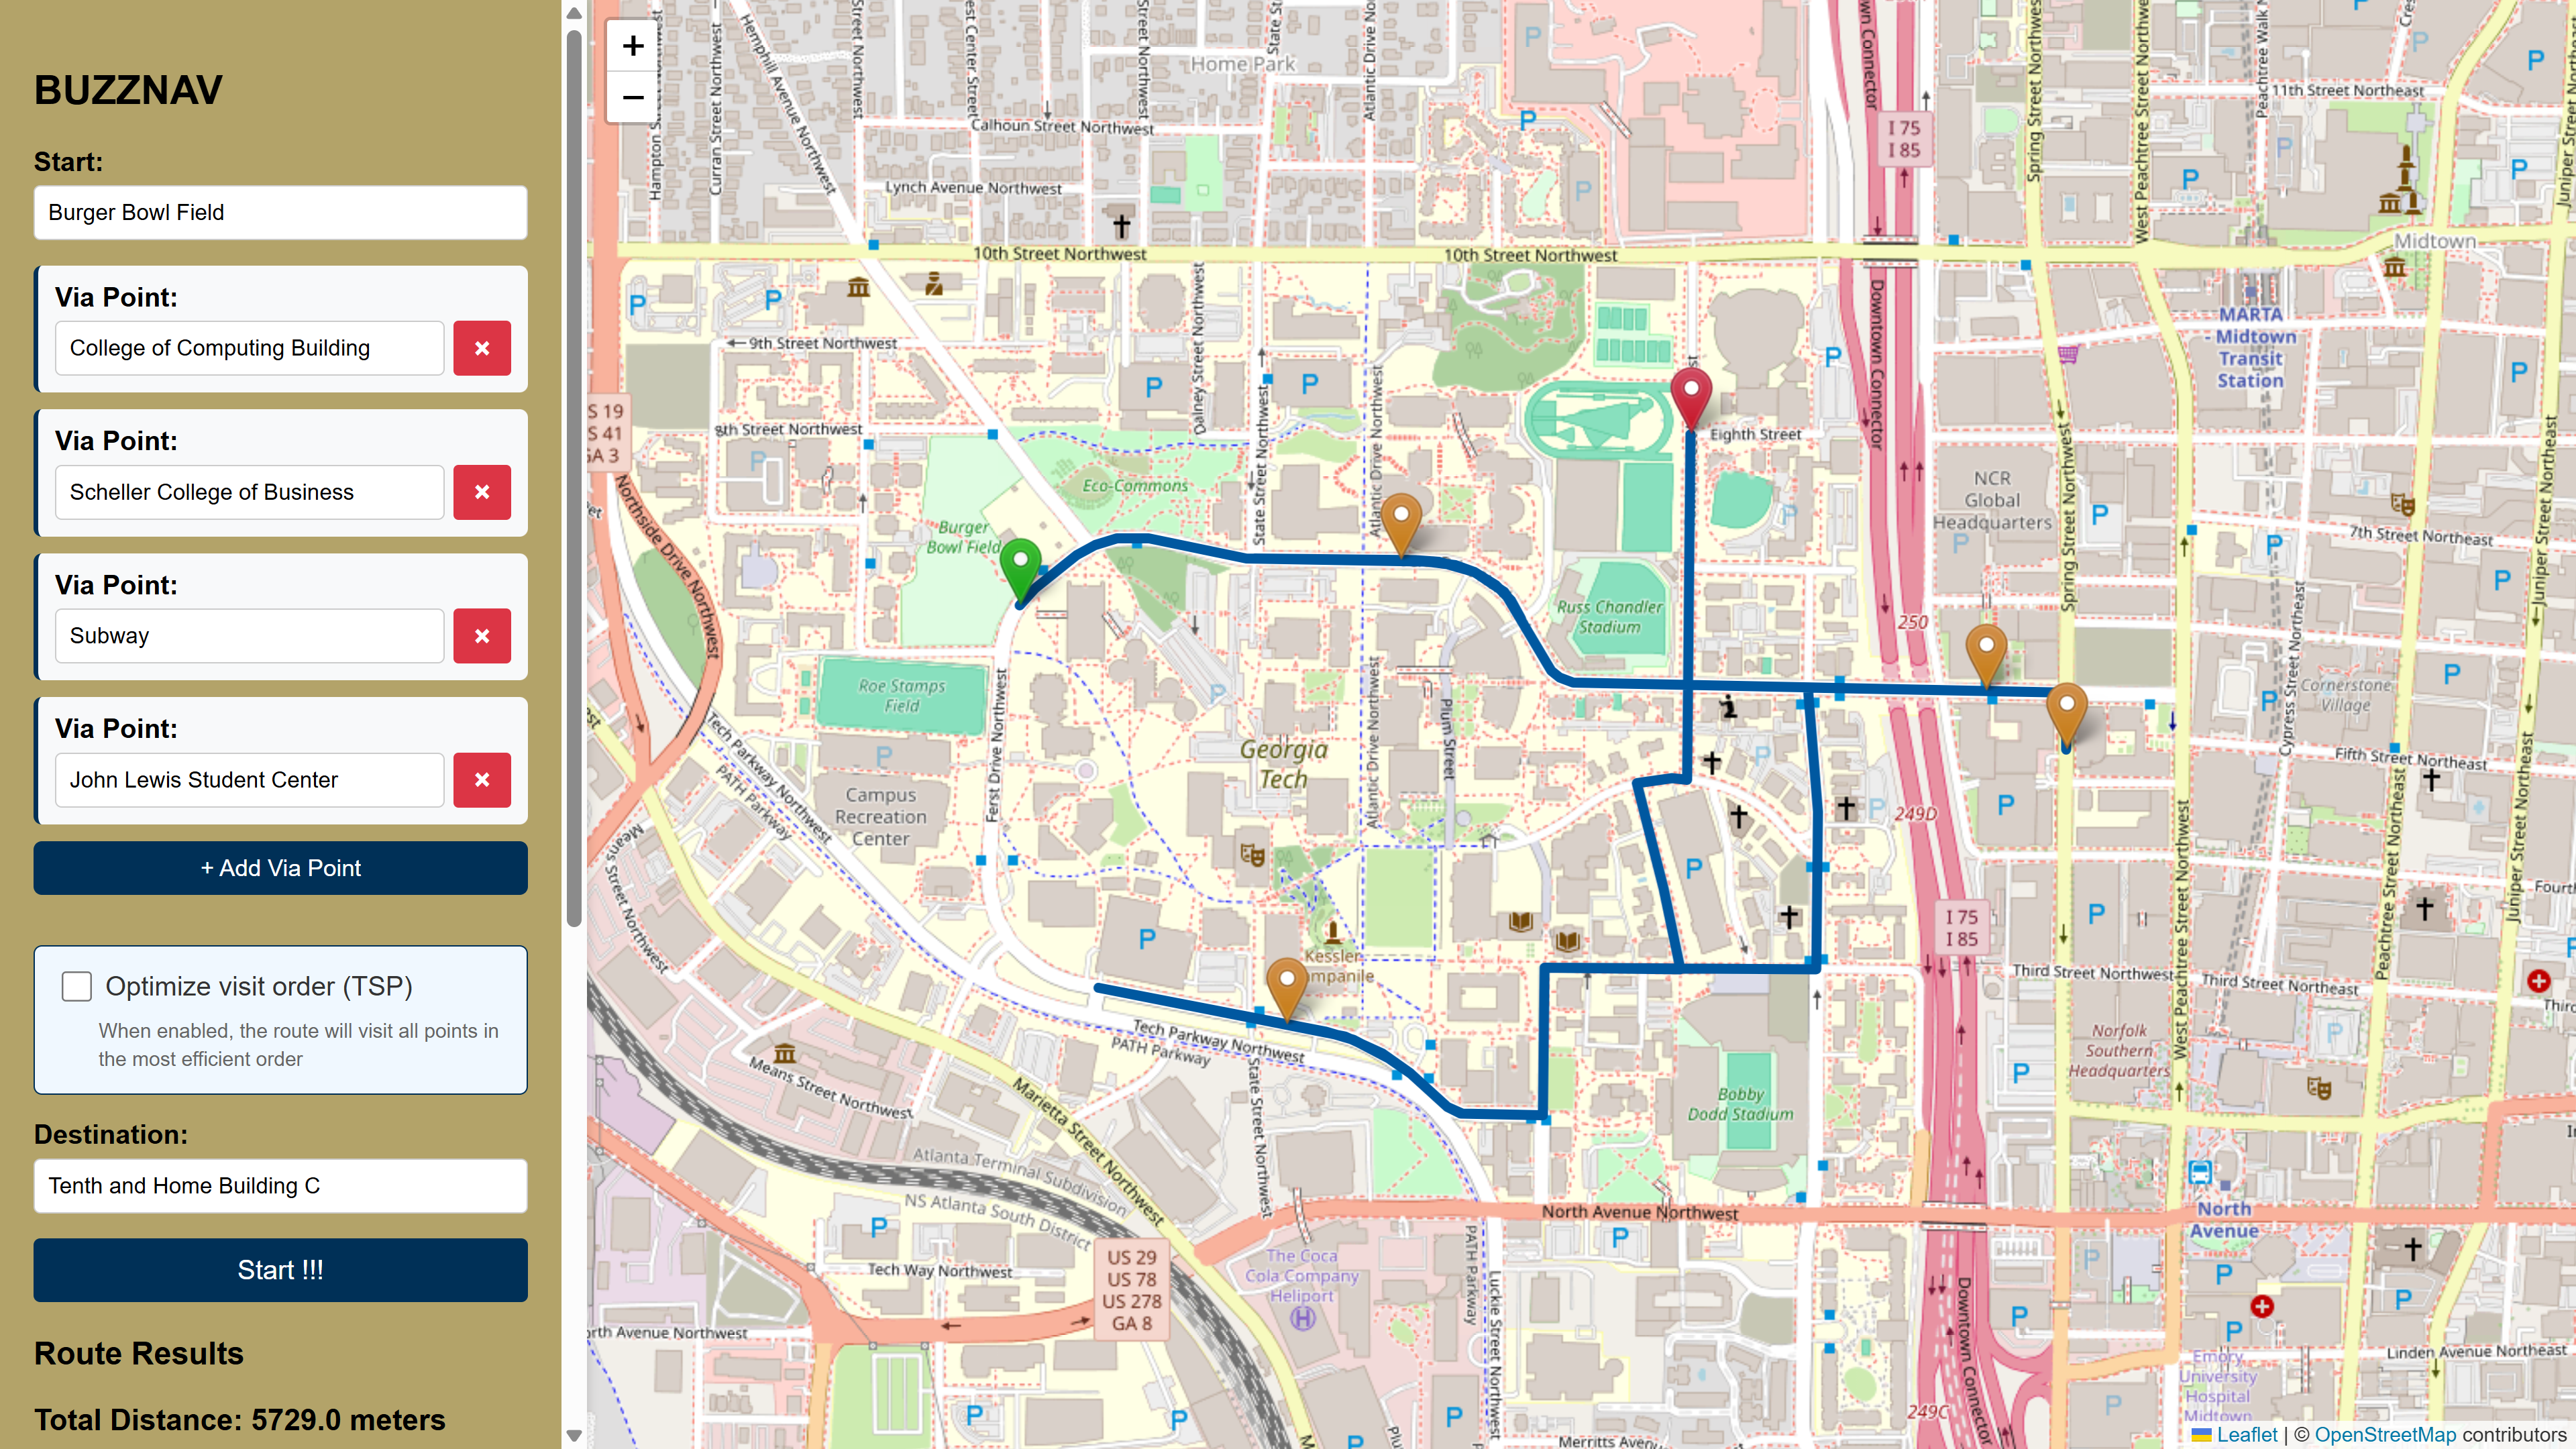
\includegraphics[width=\linewidth]{docs/Final Project Report/via.png}
        
        \caption*{(a) Via-point routing (fixed visit order)}
    \end{minipage}
    \hfill
    % Right image
    \begin{minipage}{0.48\textwidth}
        \centering
        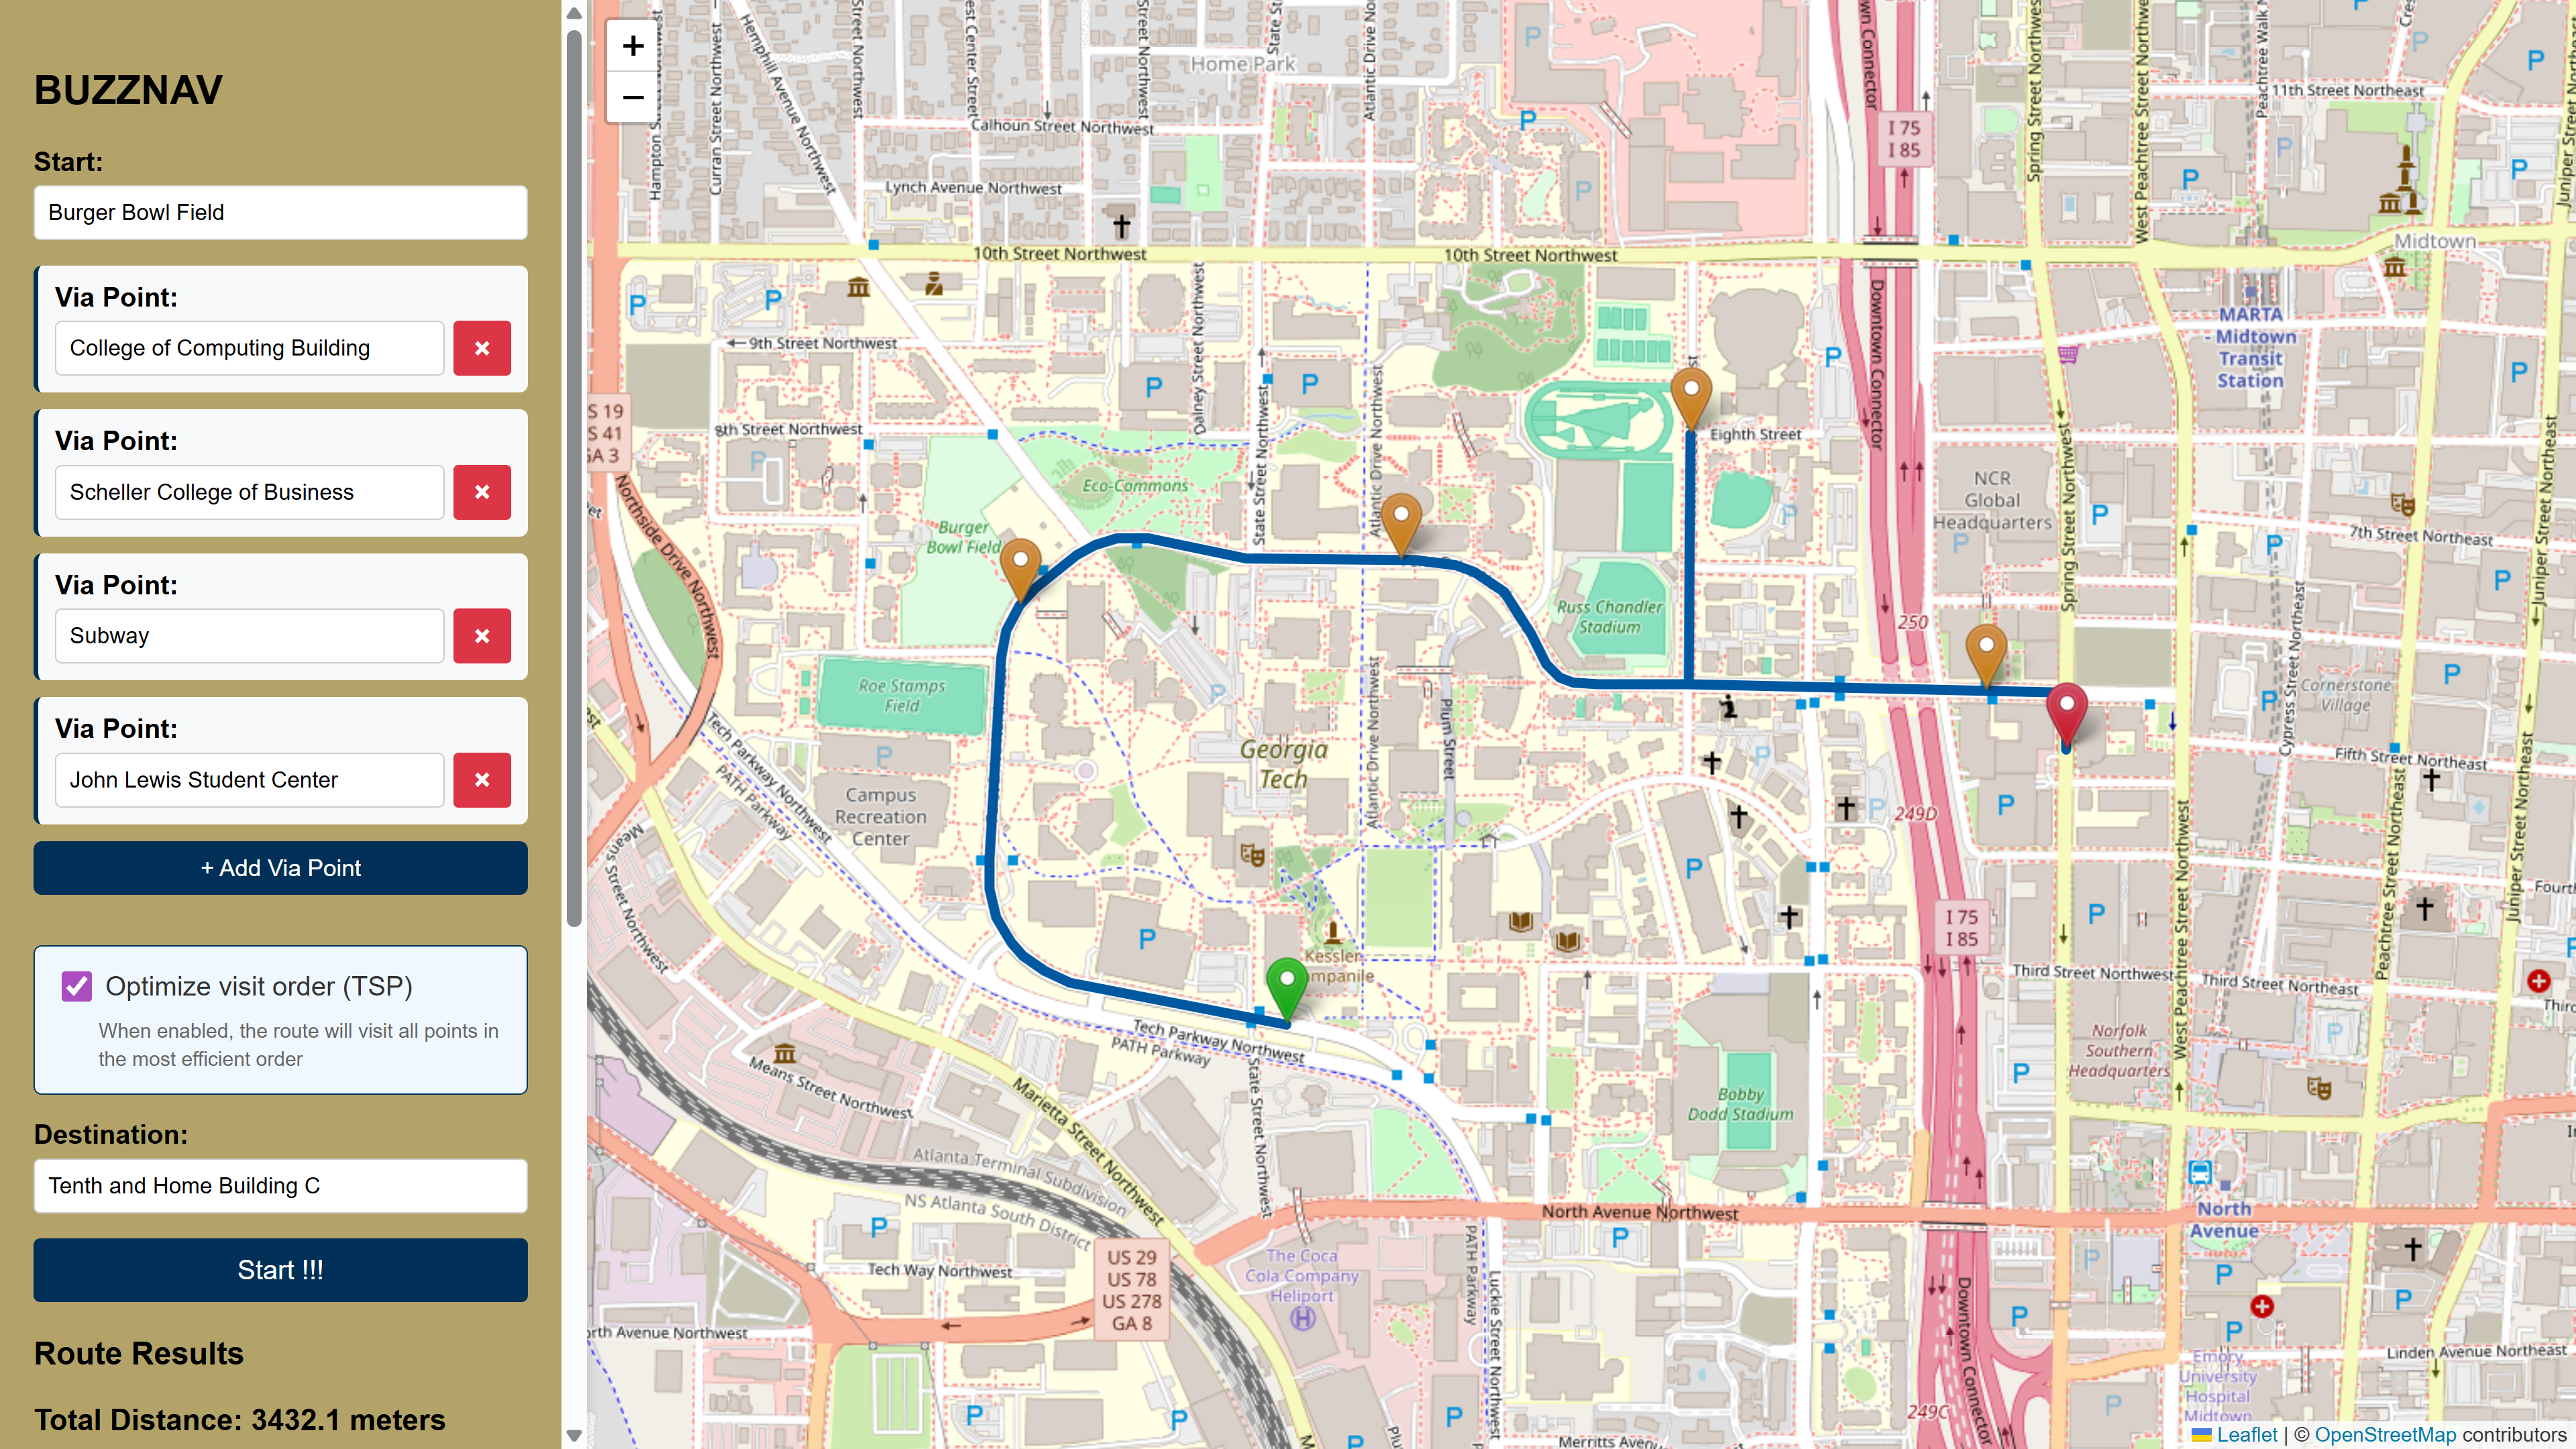
\includegraphics[width=\linewidth]{docs/Final Project Report/tsp.png}
        
        \caption*{(b) TSP-optimized visit order}
    \end{minipage}
    \caption{Comparison between fixed-order via-point routing and TSP-optimized routing.}
    \label{fig:tsp_comparison}
\end{figure*}
% ---------------------------------------------------------------

In Fig.~\ref{fig:tsp_comparison}, we compare the results of via-point routing with those of the TSP. 
Fig.~\ref{fig:tsp_comparison}(a) shows the result of visiting the given locations in order, while 
Fig.~\ref{fig:tsp_comparison}(b) shows the result of visiting the same locations without a fixed order. 
From the comparison of the visualized paths and their corresponding lengths, we can see that 
our TSP indeed finds a route that, compared with via-point routing, has fewer detours, fewer repeated segments, 
and a smaller total distance.

For users who wish to visit a set of locations without caring about the order, such as campus tourists, this feature provides substantial convenience. Moreover, the obtained results verify the correctness and practical effectiveness of the TSP optimization implemented in our system.

Our navigation system responds rapidly, returning the TSP results within 0.01\,s. 
An example run is shown below, where 12 buildings---including the \textit{Student Center}, 
\textit{Klaus Building}, \textit{the Georgia Tech Historic District}, \textit{the Georgia Tech Hotel and Conference Center}, 
\textit{the College of Business}, \textit{Starbucks}, \textit{Gold \& Bold Coffee Roasters}, \textit{Burger Bowl Field}, 
\textit{the Graduate Living Center}, \textit{Baker Building}, \textit{Georgia Tech Police}, and \textit{Russ Chandler Stadium}---are visited. 
Under 12-core parallel computation, the optimal unordered traversal of these 12 locations is computed 
in only 0.004\,s. Since in most practical scenarios the number of target nodes is fewer than 10, 
our system can be considered highly responsive.

\paragraph{Why so fast?}
First, our adjacency graph is highly sparse, and the total number of nodes is only on the order of 1{,}000. 
As a result, each run of Dijkstra's algorithm completes within approximately $10^{-6}$\,s. 
If there are $k$ locations to be visited, we only need to execute Dijkstra $k$ times to obtain all pairwise shortest-path distances.Second, after preprocessing, the remaining task reduces to determining the optimal visiting order among these $k$ nodes. Using the Held--Karp dynamic programming algorithm, the time complexity is reduced to $O(k^{2} 2^{k})$. In practical scenarios, $k$ is typically small, which keeps the exponential term manageable. 
Consequently, the overall computational workload remains limited and the system achieves very fast response times.

We can further improve the accuracy of the map and the complexity of the problem by increasing the node density. As the number of nodes increases, the computational cost will grow as well. At this point, the advantages of parallel processing become more apparent, but we may also need to consider adopting new and more advanced graph-network-related algorithms to compute the shortest paths.

\subsection{Computational Performance and Parallel Speedup}

A key objective of this project is using parallel computing to accelerate graph computation. We measured the speedup achieved by OpenMP across our main modules (i.e. the Distance Matrix construction used in TSP and the Via-Point Search).

\begin{table}[h]
\centering
\caption{Parallel Performance Speedup}
\begin{tabular}{|l|c|c|c|}
\hline
\textbf{Module} & \textbf{Cores Used} & \textbf{Algorithm} & \textbf{Speedup} \\
\hline
Distance Matrix & 8 & Parallel Dijkstra & $7.2\times$ \\
Via-Point Search & 4 & Parallel A* & $3.8\times$ \\
\hline
\end{tabular}
\label{tab:performance}
\end{table}

As summarized in Table \ref{tab:performance}:
\begin{itemize}
    \item \textbf{TSP Preprocessing:} The calculation of the all-pairs shortest path matrix, which requires running Dijkstra's algorithm $k$ times (where $k$ is the number of visiting nodes), achieved a \textbf{7.2x speedup} on an 8-core processor. This near-linear scaling indicates that single-source shortest path tasks is suitable to be parallelized.
    \item \textbf{Via-Point Segments:} The segmented A* search achieved a \textbf{3.8x speedup} on 4 cores. By decomposing the route into independent $(s \to n_1, n_1 \to n_2, \dots)$ segments, we ensured that the addition of intermediate stops does not linearly degrade system response time.
\end{itemize}

This reduction in computation time is also essential for the front-end, as it enables multi-stop queries to run interactively while maintaining a responsive user experience.

\section{Discussion and Conclusion}

\subsection{Lessons Learned}
\begin{itemize}
    \item \textbf{Choosing Appropriate Data Structures:} When constructing the node graph, since the campus network is relatively sparse, we adopted an adjacency list instead of an adjacency matrix. This not only saves storage space, but also makes it easier for us to find the neighbors of each node.

    \item \textbf{Algorithms and Algorithm Selection:} We not only became familiar with normal pathfinding algorithms taught in class, but also learned more universal method like A* and Held--Karp dynamic programming. Moreover, we got the chance to compare these algorithms' strengths and thus selected the most suitable one to solve problems. 

    \item \textbf{The Power of Parallel Computing:} Using parallel computing can greatly reduce runtime and maximize the CPU utilization.
\end{itemize}


\subsection{Practical Optimization}
Other than algorithm selection, we performed the following optimizations to ensure webpage responsiveness:
\begin{itemize}
    \item \textbf{Binary Heap Priority Queue:} In our $A^{*}$ and Dijkstra implementations, we utilized a binary heap for the priority queue. This reduced the time complexity of node retrieval from $O(V)$ to $O(\log V)$, which is critical when graph become bigger. 
    \item \textbf{Segmented Decomposition:} For the via-point routing, we treated each segment ($n_i \to n_{i+1}$) as an independent task. This design choice allowed us to map specific segments to specific CPU threads and thus execute in parallel.
    \item \textbf{Coordinate Mapping:} To speed up the communication between frontend and backend, we pre-processed the mapping of building names to Node IDs, allowing the routing engine to immediately execute graph algorithms without searching linearly on the raw dataset during runtime.
\end{itemize}

\subsection{Limitations and Tradeoffs}
Here are the limitations of BuzzNav system: 
\begin{itemize}
    \item \textbf{Held-Karp Scalability:} The Held-Karp algorithm provides an exact solution for TSP with a time complexity of $O(k^2 2^k)$. While this is highly efficient for typical campus tours (e.g., $k \leq 15$), it becomes computationally expensive as the number of destinations increases. For larger datasets ($k > 20$), a heuristic approximation would be a necessary tradeoff against optimality.
    \item \textbf{Centroid Projection Accuracy:} We linked buildings to the road network using centroid projection. In complex building geometries, this might navigates the user to a wall rather than a door.
\end{itemize}

\subsection{Future Work}
The following extensions are some possible extensions of BussNav to address current limitations:
\begin{itemize}
    \item \textbf{Accessibility Routing:} Integrating data regarding stairs/ramps would allow us to offer "Wheelchair Accessible" or "Scotter Friendly" routing options.
    \item \textbf{Indoor Navigation:} Expanding the graph to include indoor floor plans would enable navigation such as from a parking lot directly to a specific classroom number.
\end{itemize}

\subsection{Conclusion}
We demonstrates how graph algorithms can be improved via parallel computing to solve real-world navigation problems through BuzzNav. By combining the precision of $A^{*}$ for specific paths with the optimization power of Held-Karp for multi-stop tours, the system reduces travel distance by over 40\% in complex routing scenarios. The integration of a C++ backend with a responsive web frontend also proves that high-performance computing can be effectively delivered in a browser environment.

\appendix
\section{Appendix: Division of Labor}
\begin{itemize}
    \item \textbf{Algorithm \& Core Functionality}: Fred Yang, Jing He, Chia-Hsin Chiu
        \begin{itemize}
            \item Implement  A*, Dijkstra algorithms (with optional via points) and TSP optimization using Held-Karp. 
            \item Implement pathfinding api to bridge the frontend and backend. 
        \end{itemize}
    \item \textbf{Data Handling \& Graph Extensions}: Haowen Jiang, Jing He, Ming-Cheng Fan
        \begin{itemize}
            \item Improve CSV parsing robustness (e.g. check invalid edges).
            \item Integrate building entrance coordinates more accurately.
            \item Add location nodes other than buildings, such as statues, printers, restrooms, parking lot, etc.
        \end{itemize}
    \item \textbf{Routing Output \& Instructions}: Fred Yang, Ming-Cheng Fan, Haowen Jiang, Chia-Hsin Chiu
        \begin{itemize}
            \item Implement user-friendly turn-by-turn directions by replacing node\_id to building name
            \item Ensure instructions update dynamically when users change start/end points.
        \end{itemize}
    \item \textbf{Front-End UI}: Fred Yang, Chia-Hsin Chiu, Ming-Cheng Fan
        \begin{itemize}
            \item Build a user-friendly web interface to interact with the BuzzNav system using a visualized campus map.
            \item Implement interactive features such as selecting start and end locations, and adding via-points out of order.
            \item Integrate frontend with backend APIs to fetch building data and navigation paths.
            \item Format and display navigation path data clearly on the map, including markers for start, end, and via points.
        \end{itemize}
    \item \textbf{Testing, Integration \& GitHub Repository Maintenance \& Video Recording}: Team-wide
\end{itemize}

\bibliographystyle{unsrt}
\bibliography{references}

\end{document}





